\documentclass[12pt,a4paper,xcolor=dvipsnames,xcolor=table]{beamer}
 
\usepackage[utf8]{inputenc}
\usepackage[T1]{fontenc}
\usepackage{microtype}
\usepackage{libertine}
\usepackage[libertine]{newtxmath}
\usepackage[english]{babel}
\usepackage{mathtools}
\usepackage{graphicx}
\usepackage{subcaption}
%\usepackage{sourcesanspro}

% redeclare emph
\let\emph\relax % there's no \RedeclareTextFontCommand
\DeclareTextFontCommand{\emph}{\color{Blue}\em}
% beamer customizatoin
\usefonttheme[onlymath]{serif} 
\setbeamercolor{math text}{fg=Blue}
\setbeamercolor{math text displayed}{fg=Blue}
\setbeamertemplate{navigation symbols}{}
 
%Information to be included in the title page:
\title{Principal Component Analysis}
%\author{Bogdan Burlacu}
%\institute{FH Hagenberg}
\date{2017}
 
\begin{document}
 
\frame{\titlepage}
 
\begin{frame}
\frametitle{Overview}
\begin{enumerate}
    \item Eigenvectors and Eigenvalues
    \item Principal Component Analysis
    \item Practical Example 
\end{enumerate}
\end{frame}

\begin{frame}\frametitle{Eigenvectors and Eigenvalues}
A vector $v\in\mathbb{R}^n$ is an \emph{eigenvector} of a matrix $A\in\mathbb{R}^{n \times n}$ if
\[
    Av = \lambda v \tag{1}
\] where $\lambda$ is a scalar called the \emph{eigenvalue} associated with $v$.

Eigenvectors (values) are found by solving (1)
\[
    (A-\lambda I)v = 0 \tag{2} 
\]
Eq. (2) has a non-zero solution $v$ only if 
\[
    \det(A-\lambda I)=0 \tag{3}
\]
\end{frame}
\begin{frame}
\frametitle{Eigenvectors and Eigenvalues}
Example: find the eigenvectors and eigenvalues of matrix
\[
    A = 
    \begin{bmatrix}
        1 & 0\\
        1 & 3
    \end{bmatrix}
\]
Solving (3), we get
    \begin{align*}
    &~A - \lambda I = \begin{bmatrix}
        1-\lambda & 0\\
        1         & 3 -\lambda
    \end{bmatrix}\\
    & \Rightarrow \det(A-\lambda I) = (1-\lambda)(3-\lambda)\\
    & \Rightarrow \lambda_1 = 1, \lambda_2 = 3
    \end{align*}
 
Two eigenvalues $\lambda_1, \lambda_2 \Rightarrow$ two eigenvectors $v_1, v_2$.
\end{frame}

\begin{frame}
\frametitle{Eigenvectors and Eigenvalues}
Plugging $\lambda_1$ and $\lambda_2$ into (1) we have 

\begin{align*}
    \begin{bmatrix}
        1 & 0\\
        1 & 3
    \end{bmatrix}
    \begin{bmatrix}
        v_{11}\\
        v_{12} 
    \end{bmatrix} &= 1 
    \begin{bmatrix}
        v_{11}\\
        v_{12} 
    \end{bmatrix}\\
    \begin{bmatrix}
        1 & 0\\
        1 & 3
    \end{bmatrix}
    \begin{bmatrix}
        v_{21}\\
        v_{22} 
    \end{bmatrix} &= 3
    \begin{bmatrix}
        v_{21}\\
        v_{22} 
    \end{bmatrix}
\end{align*}
From which we get $v_{11} = -2 v_{12}$, $v_{21}=0$ and $v_{22}\in \mathbb{R}$. That is:
\begin{itemize}
    \item any vector $v_1 = [v_{11}~ v_{12}]^T$ where $v_{11} = -2v_{22}$ is an eigenvector of $A$ with eigenvalue $\lambda_1 = 1$. 
    \item any vector $v_2 = [v_{21}~ v_{22}]^T$ where $v_{21} = 0$ and $v_{22} \in \mathbb{R}$ is an eigenvector of $A$ with eigenvalue $\lambda_2 = 3$. 
\end{itemize}
\end{frame}

\begin{frame}
\frametitle{Eigendecomposition}
Decomposing a square matrix into its eigenvectors and eigenvalues is called \emph{eigendecomposition}.
\begin{itemize}
    \item \emph{eigenvectors} are vectors which are fixed in direction under a given linear transformation 
    \item the scaling factor of these eigenvectors is then called the \emph{eigenvalue}
\end{itemize}

Suppose we have a set of data with a certain distribution. 
\begin{itemize}
    \item eigenvectors $v_i$ tell us the orientation of the distribution
    \item eigenvalues $\lambda_i$ tell the variance in each dimension
\end{itemize}   
\end{frame}

\begin{frame}
\frametitle{Eigendecomposition}
\[
    \Sigma = \begin{bmatrix}
        0.3 & 0.2\\
        0.2 & 0.3
    \end{bmatrix},~
    v = \begin{bmatrix}
        0.707 & -0.707\\
        0.707 & 0.707
    \end{bmatrix},~
    \lambda = \begin{bmatrix}
        0.5\\
        0.1
    \end{bmatrix}
\]
    \centering
    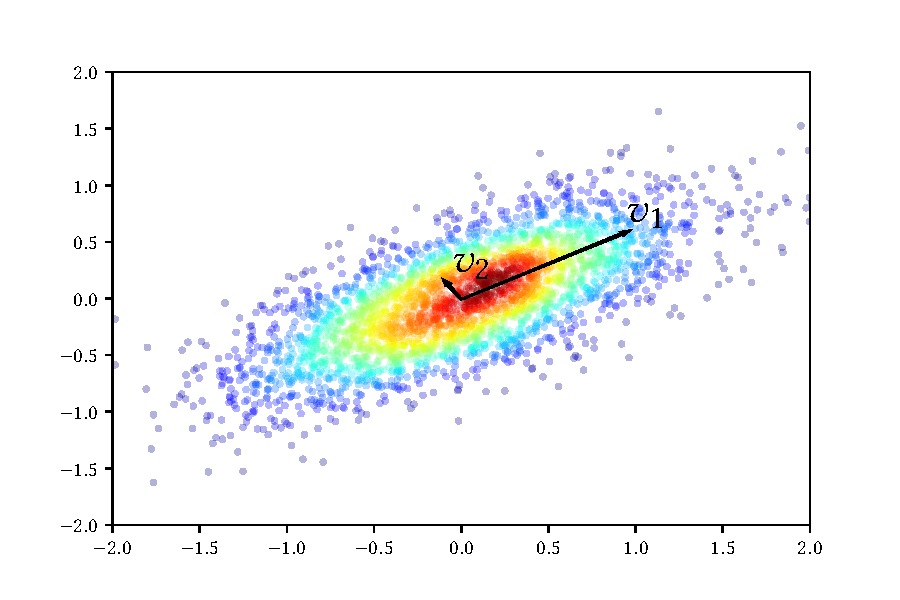
\includegraphics[width=1\textwidth]{fig/2d_distribution}
\end{frame}

\begin{frame}
\frametitle{Principal Component Analysis}
    \begin{itemize}
    \item Reduce the dimensionality of the original feature set by projecting onto a smaller subspace, where the \emph{eigenvectors} will form the axes.    
    \item We use the corresponding \emph{eigenvalues} to choose which dimensions to include. The new dimensions are \emph{principal components}.
\end{itemize}
\end{frame}

\begin{frame}
\frametitle{Principal Component Analysis}
\framesubtitle{Example: Iris Dataset}
    \begin{itemize}
        \item R. A. Fisher, \textit{The Use of Multiple Measurements in Taxonomic Problems}, 1936
        \item Data describing the morphologic variation of Iris flowers of three related species (three class labels) 
        \item Four features: the length and width of the sepals and petals, in centimeters
    \end{itemize}
    \begin{figure}
        \centering
        \begin{subfigure}{0.3\textwidth}
            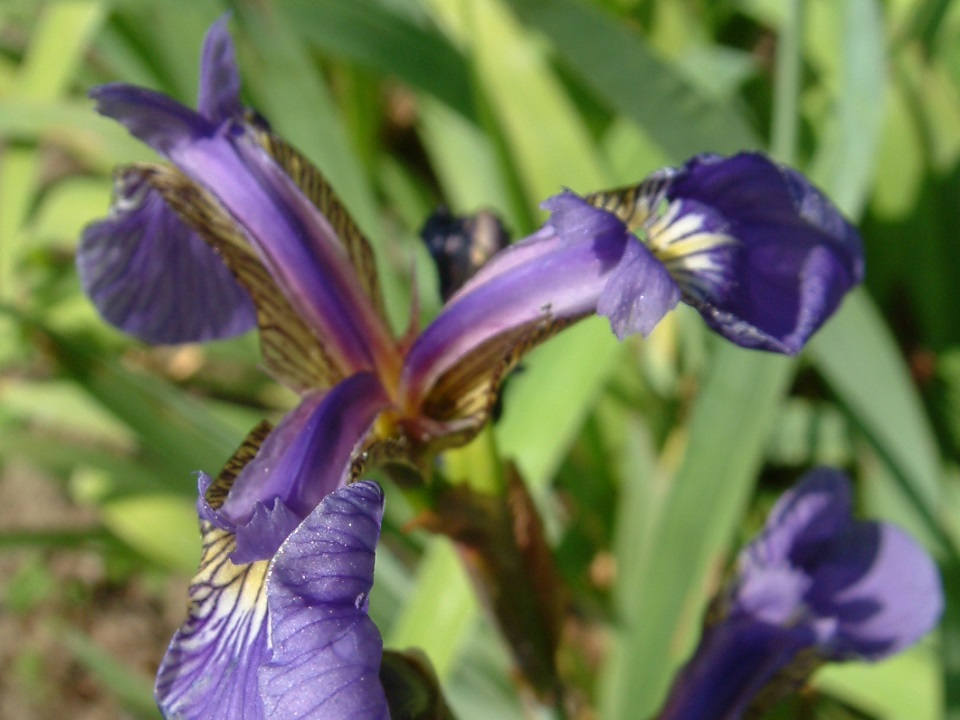
\includegraphics[width=\textwidth]{fig/iris_setosa.jpg}\caption{Iris-setosa}
        \end{subfigure}
        \begin{subfigure}{0.3\textwidth}
            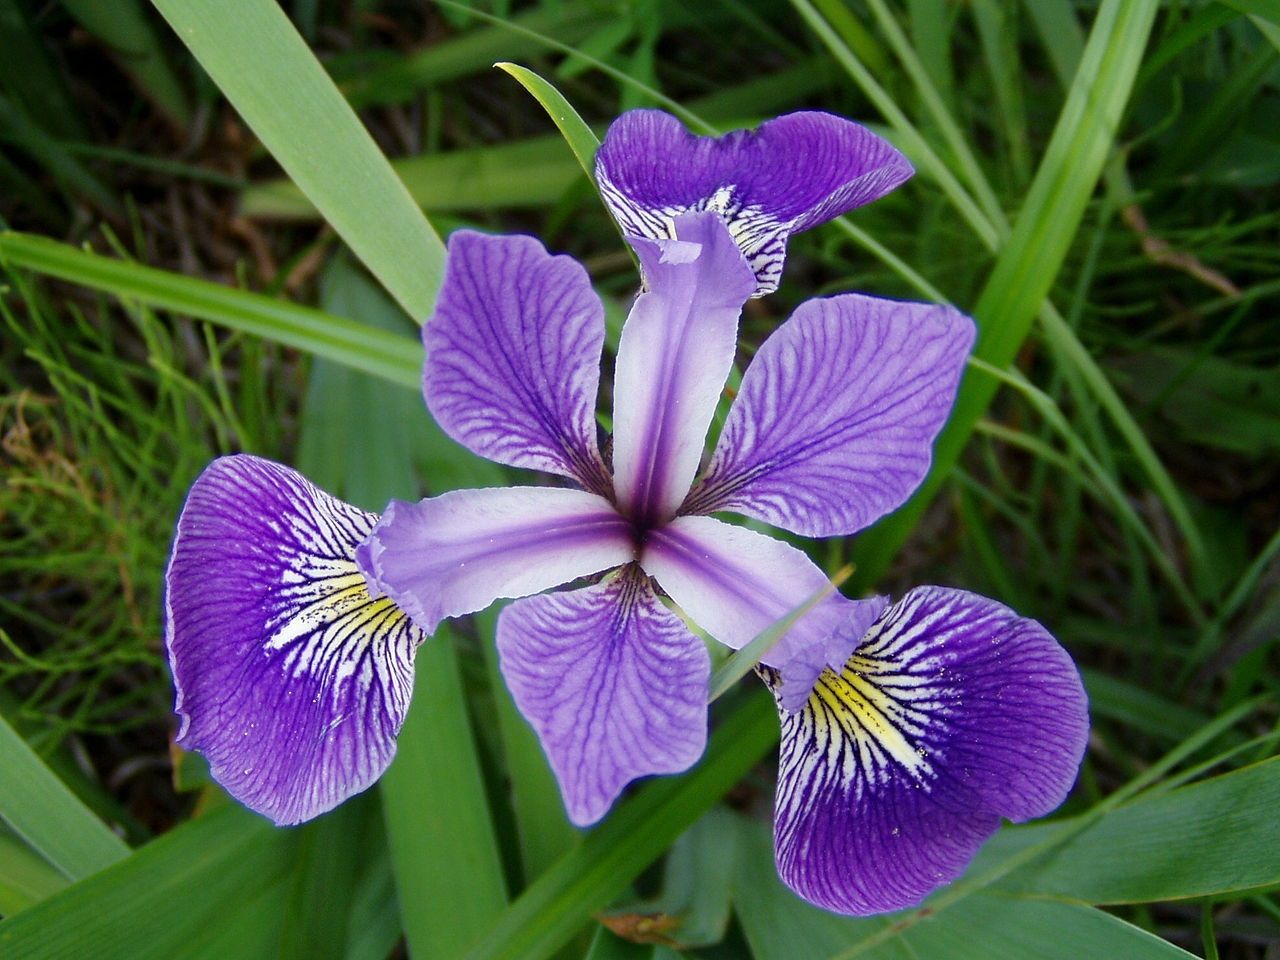
\includegraphics[width=\textwidth]{fig/iris_versicolor.jpg}\caption{Iris-versicolor}
        \end{subfigure}
        \begin{subfigure}{0.3\textwidth}
            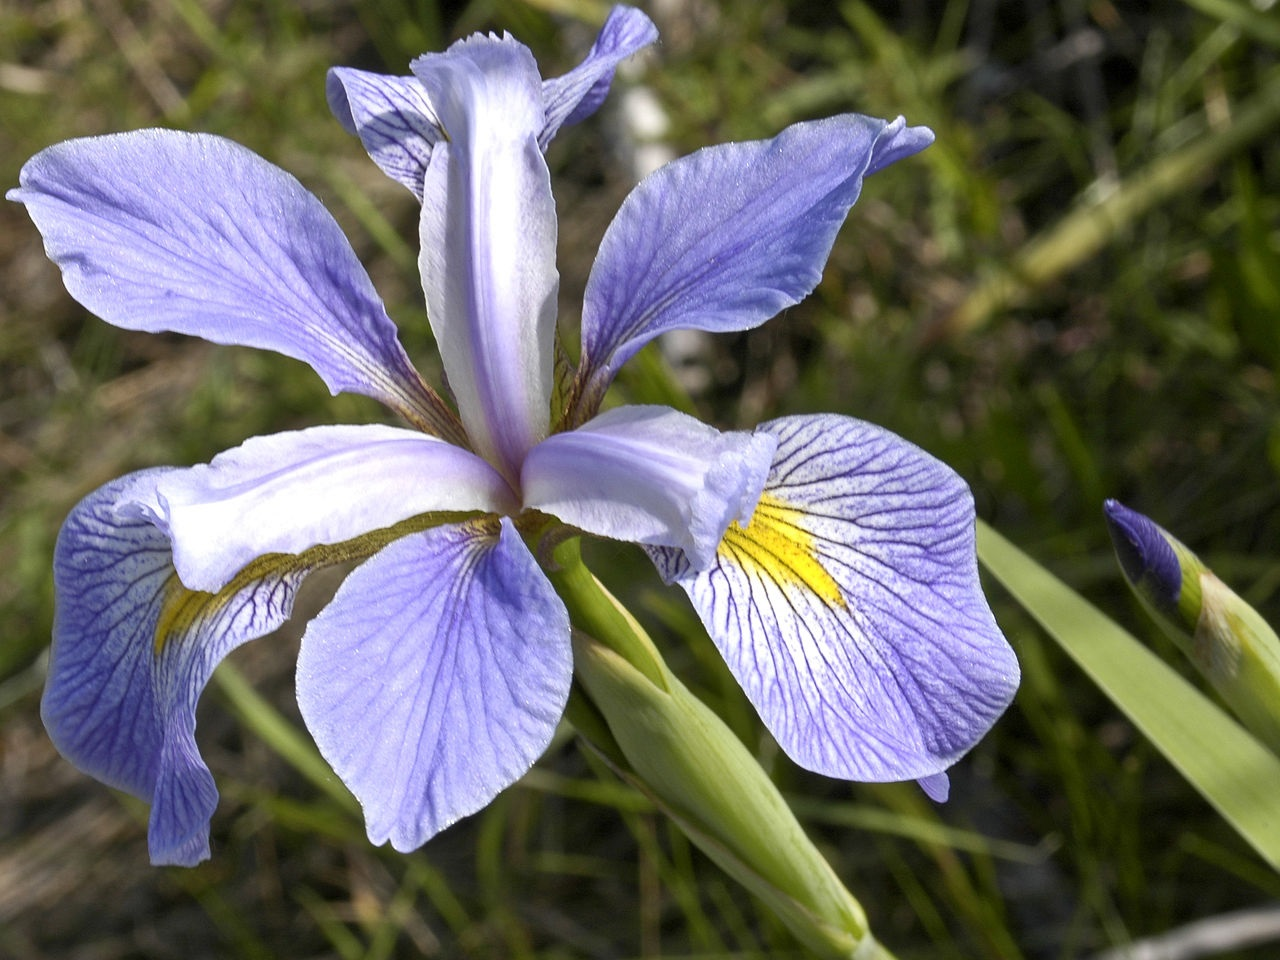
\includegraphics[width=\textwidth]{fig/iris_virginica.jpg}\caption{Iris-virginica}
        \end{subfigure} 
        {\color{gray} (source: https://en.wikipedia.org/wiki/Iris\_flower\_data\_set)}
    \end{figure}
\end{frame}

\begin{frame}
\frametitle{Principal Component Analysis}
\framesubtitle{Example: Iris Dataset}

Input data $\mathbf{X}$
\[
    \mathbf{x}^T = \begin{bmatrix}
        x_1\\ x_2\\ x_3 \\x_4
    \end{bmatrix} = \begin{bmatrix*}[l]
        \text{Sepal length}\\ \text{Sepal width}\\ \text{Petal length}\\ \text{Petal width}
    \end{bmatrix*}
\]
\begin{itemize}
    \item 150 instances (50 for each class), no missing values
    \item Predicted attribute: species
\end{itemize}
\end{frame}

\begin{frame}
\frametitle{Principal Component Analysis}
\framesubtitle{Example: Iris Dataset}
    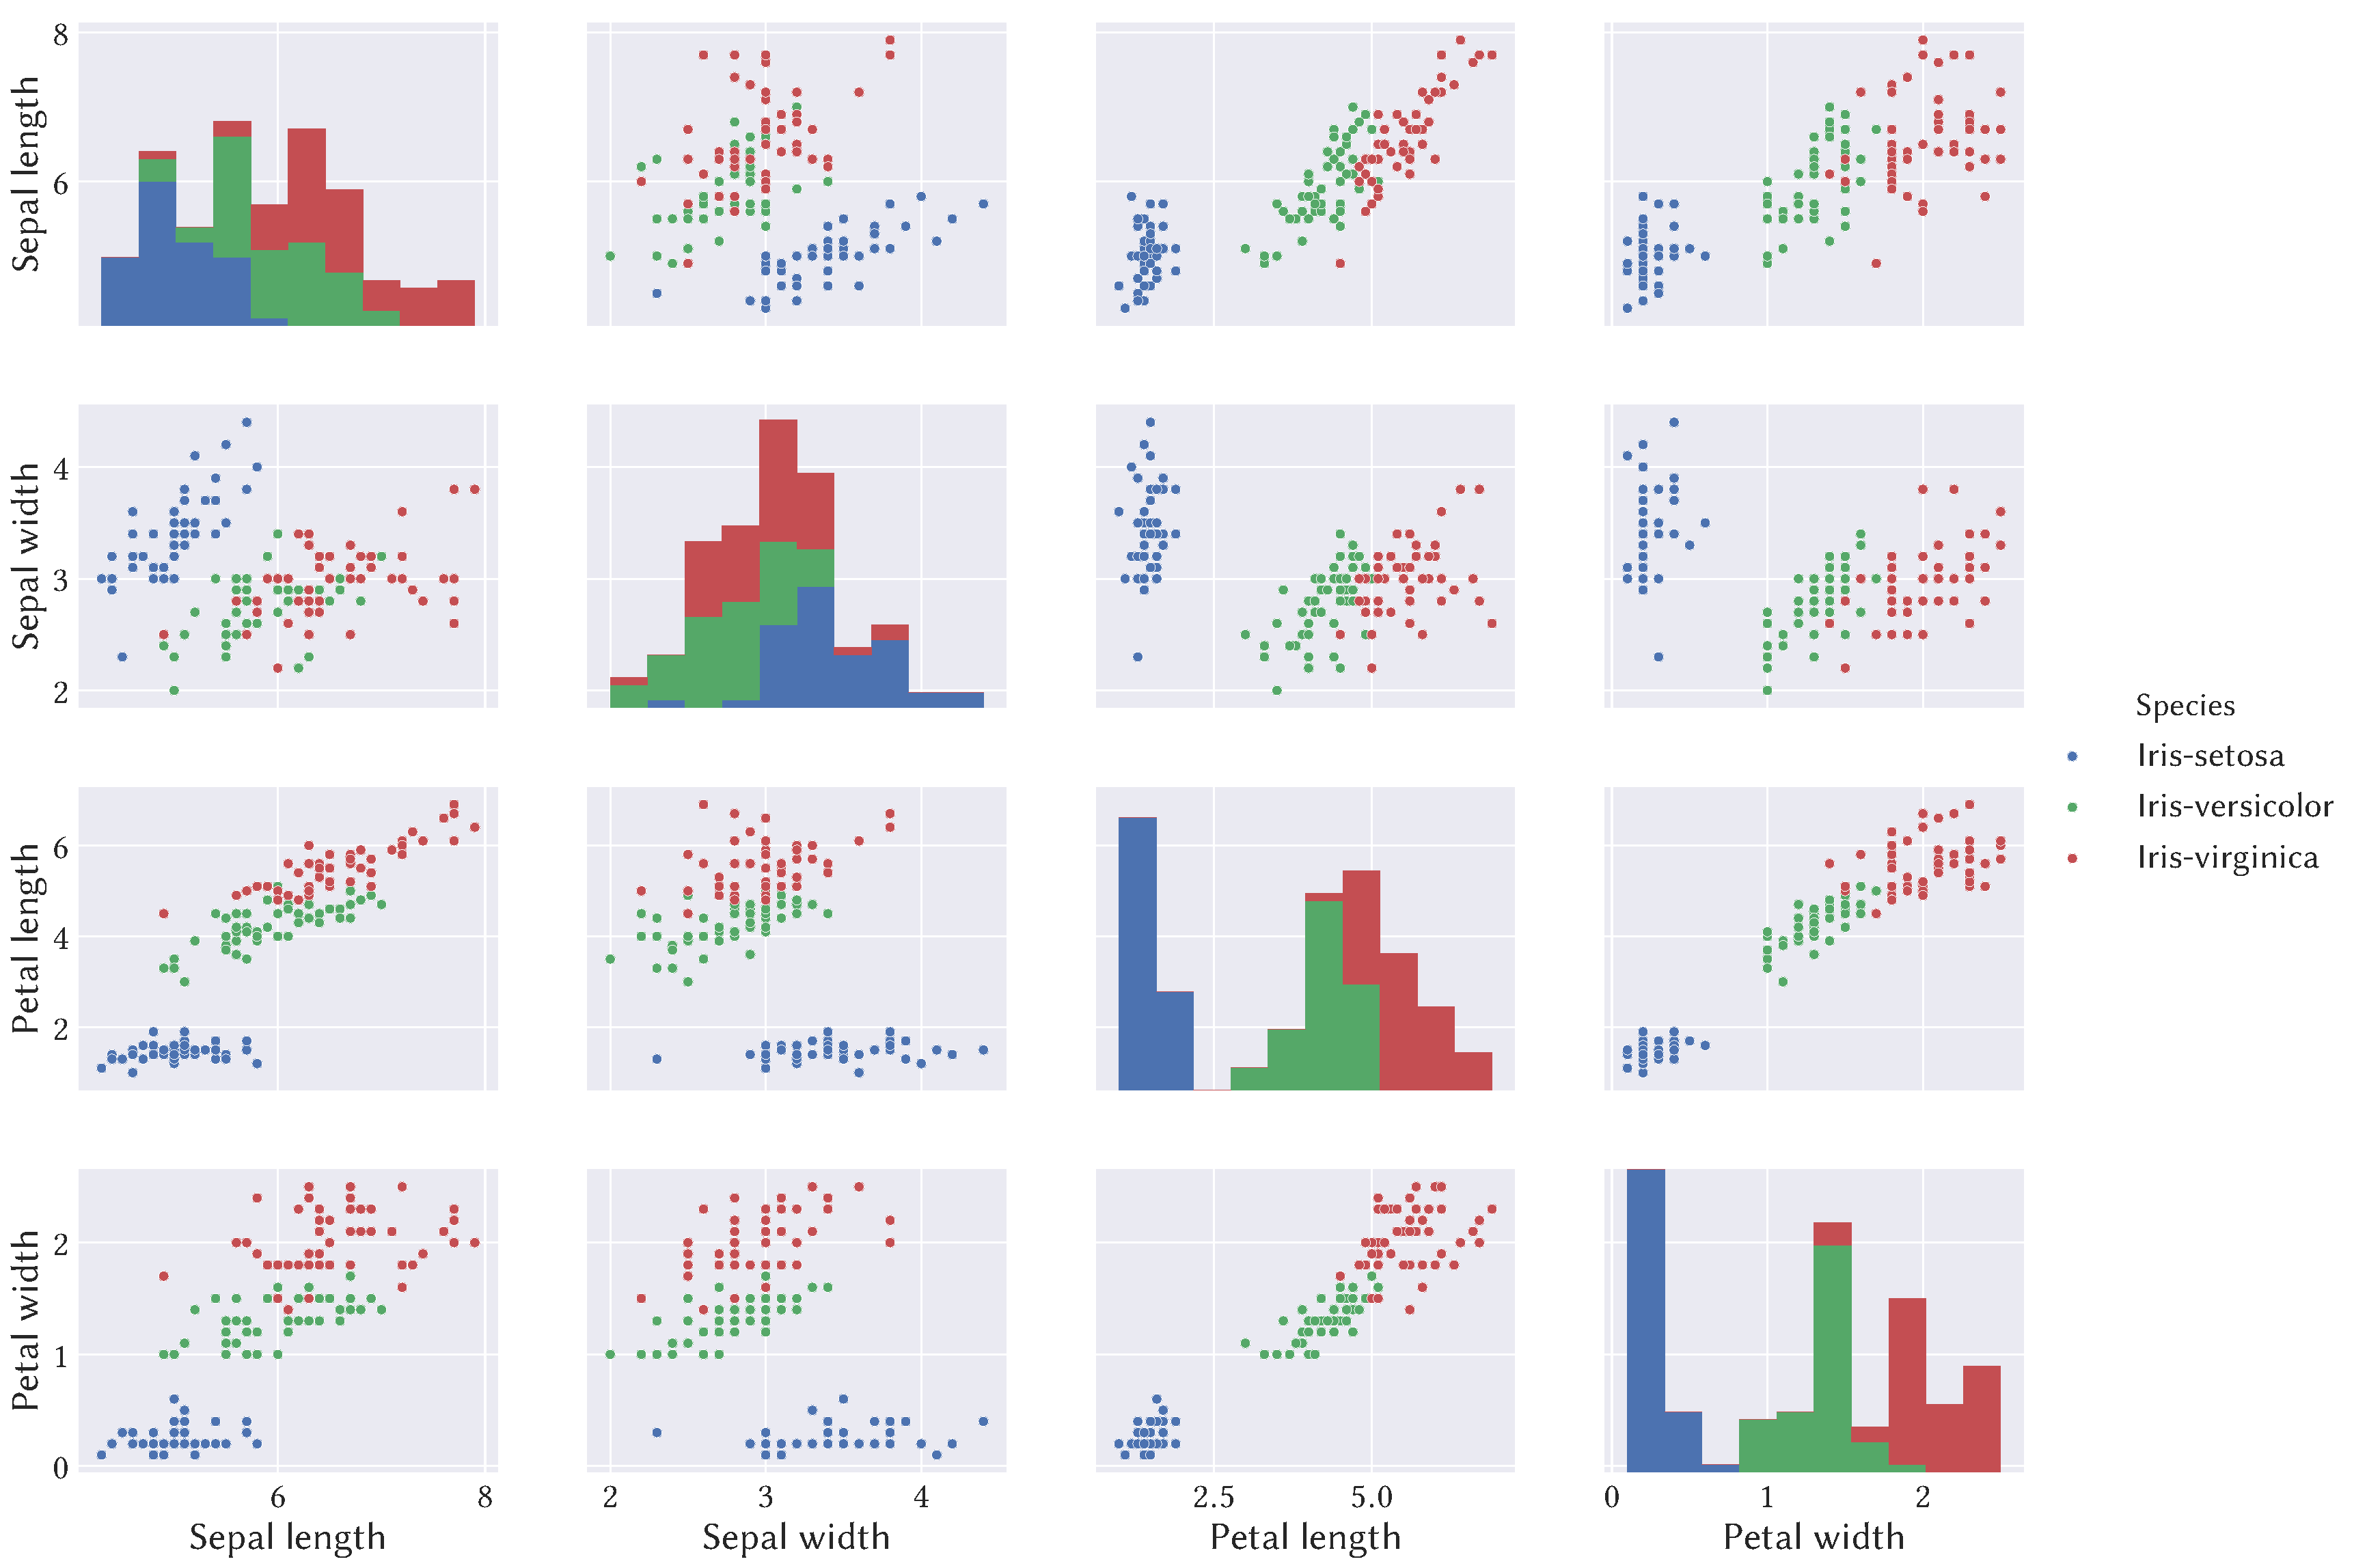
\includegraphics[width=1.1\textwidth]{fig/iris_scatter}
\end{frame}

\begin{frame}
\frametitle{Principal Component Analysis}
\framesubtitle{Example: Iris Dataset}
    Step-by-step guide
    \begin{enumerate}
        \item Standardize the data (mean = 0, variance = 1) 
        \item Calculate \emph{eigenvectors} and \emph{eigenvalues}
        \item Choose $k$ principal components based on the $k$ largest \emph{eigenvalues}
        \item Construct projection matrix $\mathbf{W}$ from the selected $k$ \emph{eigenvectors}
        \item Transform original feature space $\mathbf{X}$ using $\mathbf{W}$ to obtain $k$-dimensional feature subspace $\mathbf{Y}$
            \[
                \overbrace{\mathbf{Y}}^{\text{Projected data}} = \underbrace{\mathbf{X}}_{\text{Original data}} \cdot \overbrace{\mathbf{W}}^{\text{Projection matrix}}
                \]
    \end{enumerate}
\end{frame}

\begin{frame}[t]
\frametitle{Principal Component Analysis}
\framesubtitle{Example: Iris Dataset}
    1. Standardization (Z-score normalization)
    \begin{itemize}
        \item Transform the data to have zero mean and unit variance 
            \[
                x' = \frac{x - \mu}{\sigma}
            \]
    \item Important step for many machine learning algorithms (eg., k-means, k-NN, SVM, LDA, PCA, logistic regression)
    \item When in doubt, standardize
    \end{itemize}
\end{frame}

\begin{frame}[t]
\frametitle{Principal Component Analysis}
\framesubtitle{Example: Iris Dataset}
    2. Eigenvectors and eigenvalues
    \begin{itemize}
         \item Eigendecomposition of covariance matrix $\Sigma$, where 
             \[
                 \sigma_{jk} = \frac{1}{n-1}\sum_{i=1}^{n}(x_{ij}-\overline{x}_j)(x_{ik}-\overline{x}_k)
             \]
     \item We can also use the correlation matrix $\mathrm{corr}(\mathbf{X})$ where 
         \[
             r_{jk} = \frac{\sum_{i=1}^{n}(x_{ij}-\overline{x}_j)(x_{ik}-\overline{x}_k)}{(n-1)s_j s_k}   
         \]
         
         %$\mathrm{corr}(\mathbf{X})=(\mathrm{diag}(\Sigma))^\frac{1}{2} \Sigma (\mathrm{diag}(\Sigma))^\frac{1}{2}$
         \item In practice, we prefer singular value decomposition (computationally more efficient) over eigendecomposition
    \end{itemize}
\end{frame}

\begin{frame}[t]
\frametitle{Principal Component Analysis}
\framesubtitle{Example: Iris Dataset}
    2. Eigenvectors and eigenvalues
    \begin{align*}
        \Sigma &= \begin{bmatrix}
            1.0067 & -0.1101 & 0.8776 & 0.8234\\
            -0.1101 & 1.0067 & -0.4233 & -0.3589\\  
            0.8776 & -0.4233 & 1.0067 & 0.9692\\
            0.8234 & -0.3589 & 0.9692 & 1.0067
        \end{bmatrix}\\
        V &= \begin{bmatrix}
            0.5224 & -0.3723 & -0.7210 & 0.2620\\
            -0.2634 & -0.9256 & 0.2420 & -0.1241\\
            0.5813 & -0.0211 & 0.1409 & -0.8012\\
            0.5656 & -0.0654 & 0.6338 & 0.5235
        \end{bmatrix}, \lambda = \begin{bmatrix}
            2.9304\\ 0.9274\\ 0.1483\\ 0.0207
        \end{bmatrix}^T
    \end{align*}
    \begin{itemize}
        \item Four dimensions $\to$ four eigen vector/value pairs
        \item Lamba values represent the amount of variance explained by each principal component 
    \end{itemize}
\end{frame}

\begin{frame}[t]
    \frametitle{Principal Component Analysis}
    \framesubtitle{Example: Iris Dataset}
    3. Choosing principal components (PC1 and PC2)
    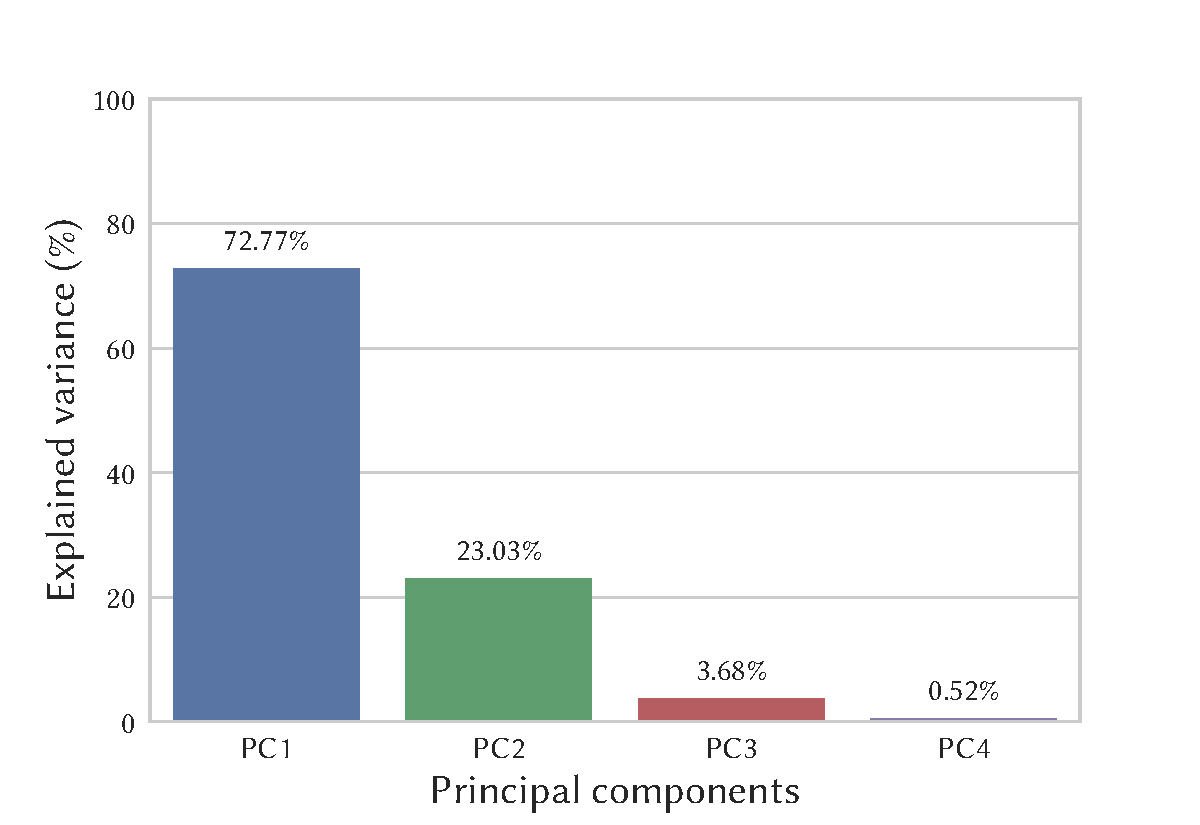
\includegraphics[width=1\textwidth]{fig/iris_principal_components}
\end{frame}

\begin{frame}[t]
    \frametitle{Principal Component Analysis}
    \framesubtitle{Example: Iris Dataset}
    4. Construct the projection matrix
    \begin{itemize}
        \item We keep the first two \emph{eigenvectors} corresponding to the two principal components, and we obtain
            \[
                \mathbf{W} = \begin{bmatrix}
                    0.5224 & -0.3723\\
                    -0.2634 & -0.9256\\
                    0.5813 & -0.0211\\
                    0.5656 & -0.0654 
                \end{bmatrix}
                \]
    \end{itemize}
    5. Project the feature space
    \[ 
        \mathbf{Y} = \mathbf{X} \mathbf{W}  
    \]
\end{frame}

\begin{frame}[t]
    \frametitle{Principal Component Analysis}
    \framesubtitle{Example: Iris Dataset}
    Samples scatterplot in the lower-dimensional feature space
    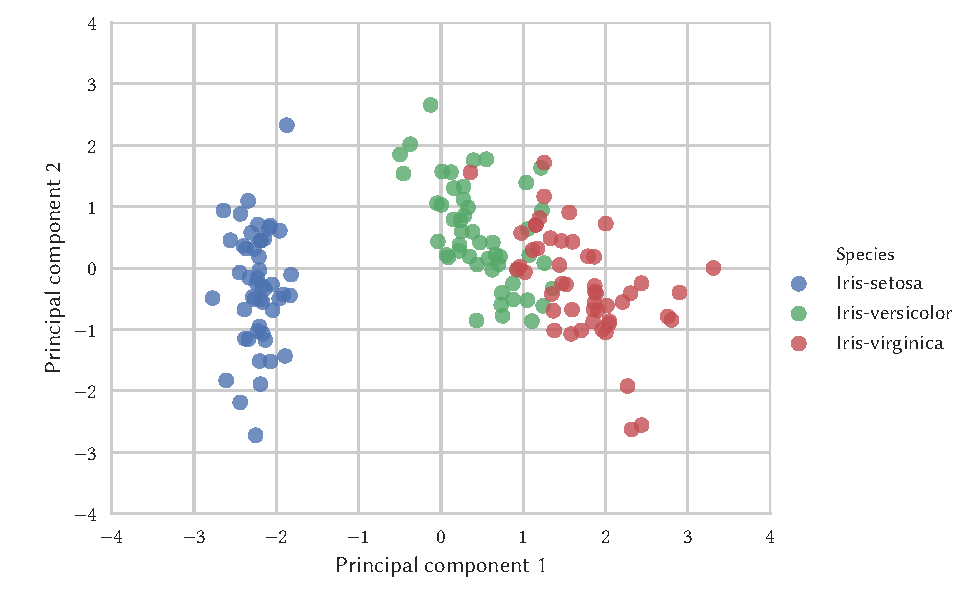
\includegraphics[width=1\textwidth]{fig/iris_principal_components_scatter}
\end{frame}

\begin{frame}
    \frametitle{Principal Component Analysis}
    \framesubtitle{Example: Iris Dataset}
    Contribution of original features to each principal component 
    \centering
    \begin{figure}
        \begin{tabular}{|l|c|c|}
            \hline
            & Principal component 1 & Principal component 2\\
            \hline
            \hline
            Sepal length & 79.43\% & 12.77\% \\
            Sepal width & 20.19\% & 78.92\% \\
            Petal length & 98.34\% & 0.04\% \\
            Petal width & 93.12\% & 0.39\% \\
            \hline
        \end{tabular}
    \end{figure}
\end{frame}
\end{document}
